\documentclass[11pt]{article}
\usepackage[margin=3cm]{geometry}
\usepackage[italian]{babel}
\usepackage[hidelinks]{hyperref}
\usepackage{amsmath}
\usepackage{graphicx}
\usepackage[nameinlink, noabbrev, capitalise, italian]{cleveref}
\usepackage{enumitem}
\usepackage{caption}
\usepackage{float}
\usepackage{amsmath}
\usepackage[ruled, vlined, linesnumbered]{algorithm2e}
\SetAlgorithmName{Algoritmo}{Algoritmo}{Elenco degli algoritmi}
\crefname{algocf}{Algoritmo}{Algoritmo}

\tolerance=1
\emergencystretch=\maxdimen
\hyphenpenalty=10000
\hbadness=10000
\setlength\parindent{0pt}

\def\gmaps{\textit{Google Maps}}

\begin{document}
\begin{titlepage}
    \begin{center}
        \vspace*{5cm}
            
        \Huge
        \textbf{Cellular Connectivity and\\Noise Map}
            
        \vspace{0.5cm}
        \LARGE
        Relazione
            
        \vspace{1cm}
          
		\hfill
		\begin{center}
        	{\large{\bf Xia $\cdot$ Tian Cheng}}\\[-0.2em]
			{\large Matricola: \texttt{0000975129}}\\[-0.2em]
			{\large Email: tiancheng.xia@studio.unibo.it}
        \end{center}
            
        \vspace{4cm}
            
        Anno accademico\\
        $2022 - 2023$
            
        \vspace{0.8cm}
            
            
        \Large
        Corso di Laboratorio di applicazioni mobili\\
        Alma Mater Studiorum $\cdot$ Università di Bologna\\
            
    \end{center}
\end{titlepage}
\newpage

\pagenumbering{roman}
\tableofcontents
\newpage

\pagenumbering{arabic}


\section{Introduzione}

\subsection{Feature implementate}

Di seguito sono elencate le feature implementate:
\begin{itemize}
    \item Mappa partizionata in aree non sovrapposte con ridimensionamento automatico delle celle in base al livello dello zoom (\cref{fig:overview_map}).
    \item Range della qualità delle misurazioni calcolato automaticamente, con possibilità di scegliere il numero di classi da creare (\cref{fig:overview_ranges}).
    \item Misurazione di Wi-Fi, LTE, rumore e Bluetooth con le seguenti modalità:
    \begin{itemize}[topsep=0pt]
        \item Attiva su comando dell'utente.
        \item Passiva dopo un determinato intervallo temporale o durante il movimento. 
        \item In background durante il movimento.
    \end{itemize}
    \item Filtro di ricerca per alcune tipologie di misurazioni (Wi-Fi e Bluetooth)
    \item Notifiche per aree prive di misurazioni recenti.
    \item Esportazione su file e importazione delle misurazioni (\cref{fig:overview_import_export}).
\end{itemize}


\subsection{Screenshot applicazione}

\begin{figure}[H]
    \centering
    \begin{minipage}[b]{0.25\textwidth}
      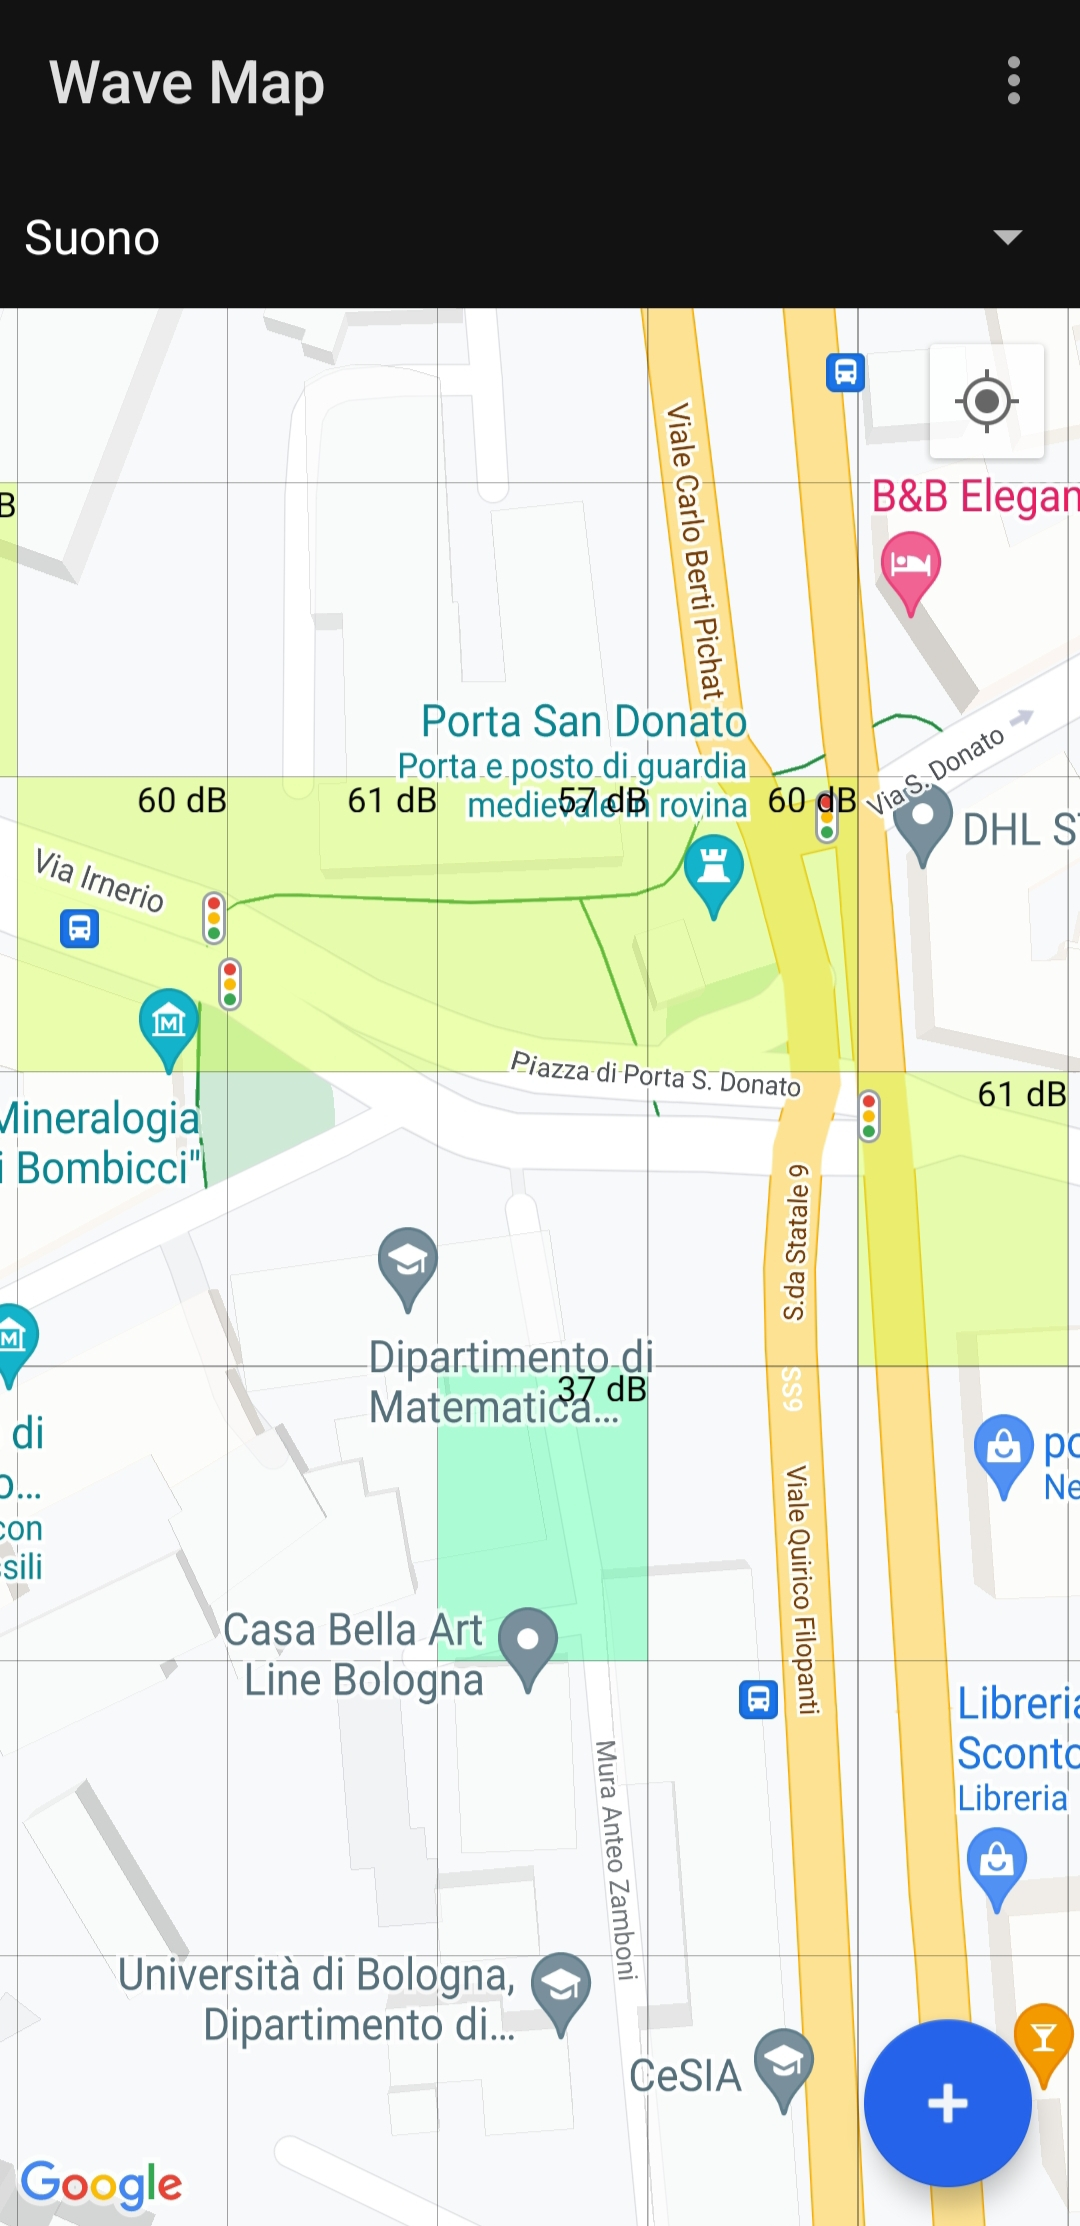
\includegraphics[width=\textwidth]{./img/overview/map_zoom1.jpg}
    \end{minipage}
    \hspace*{1cm}
    \begin{minipage}[b]{0.25\textwidth}
      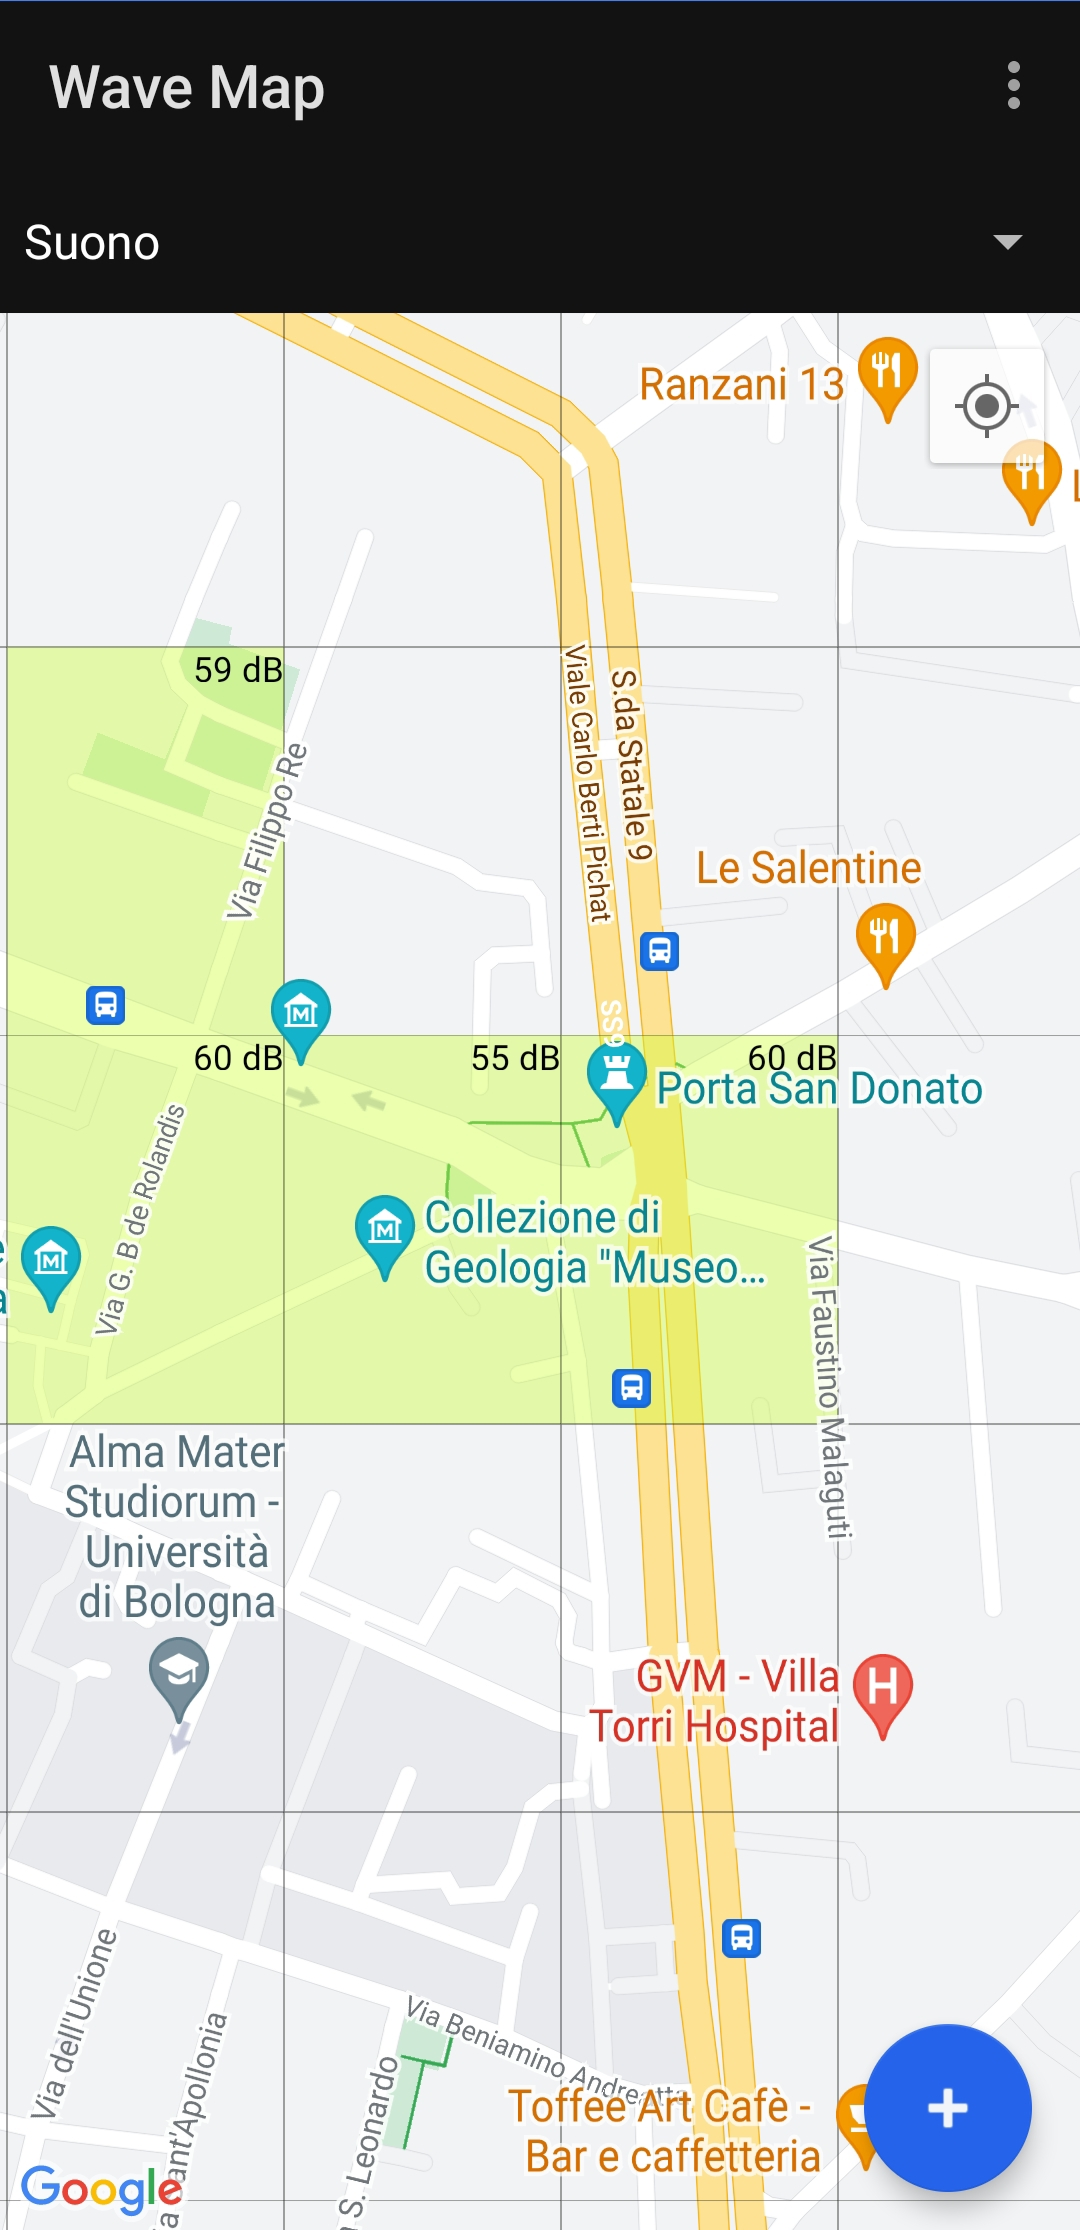
\includegraphics[width=\textwidth]{./img/overview/map_zoom2.jpg}
    \end{minipage}
    \caption{Mappa con celle ridimensionate automaticamente} \label{fig:overview_map}
\end{figure}

\begin{figure}[H]
    \centering
    \begin{minipage}[b]{0.25\textwidth}
      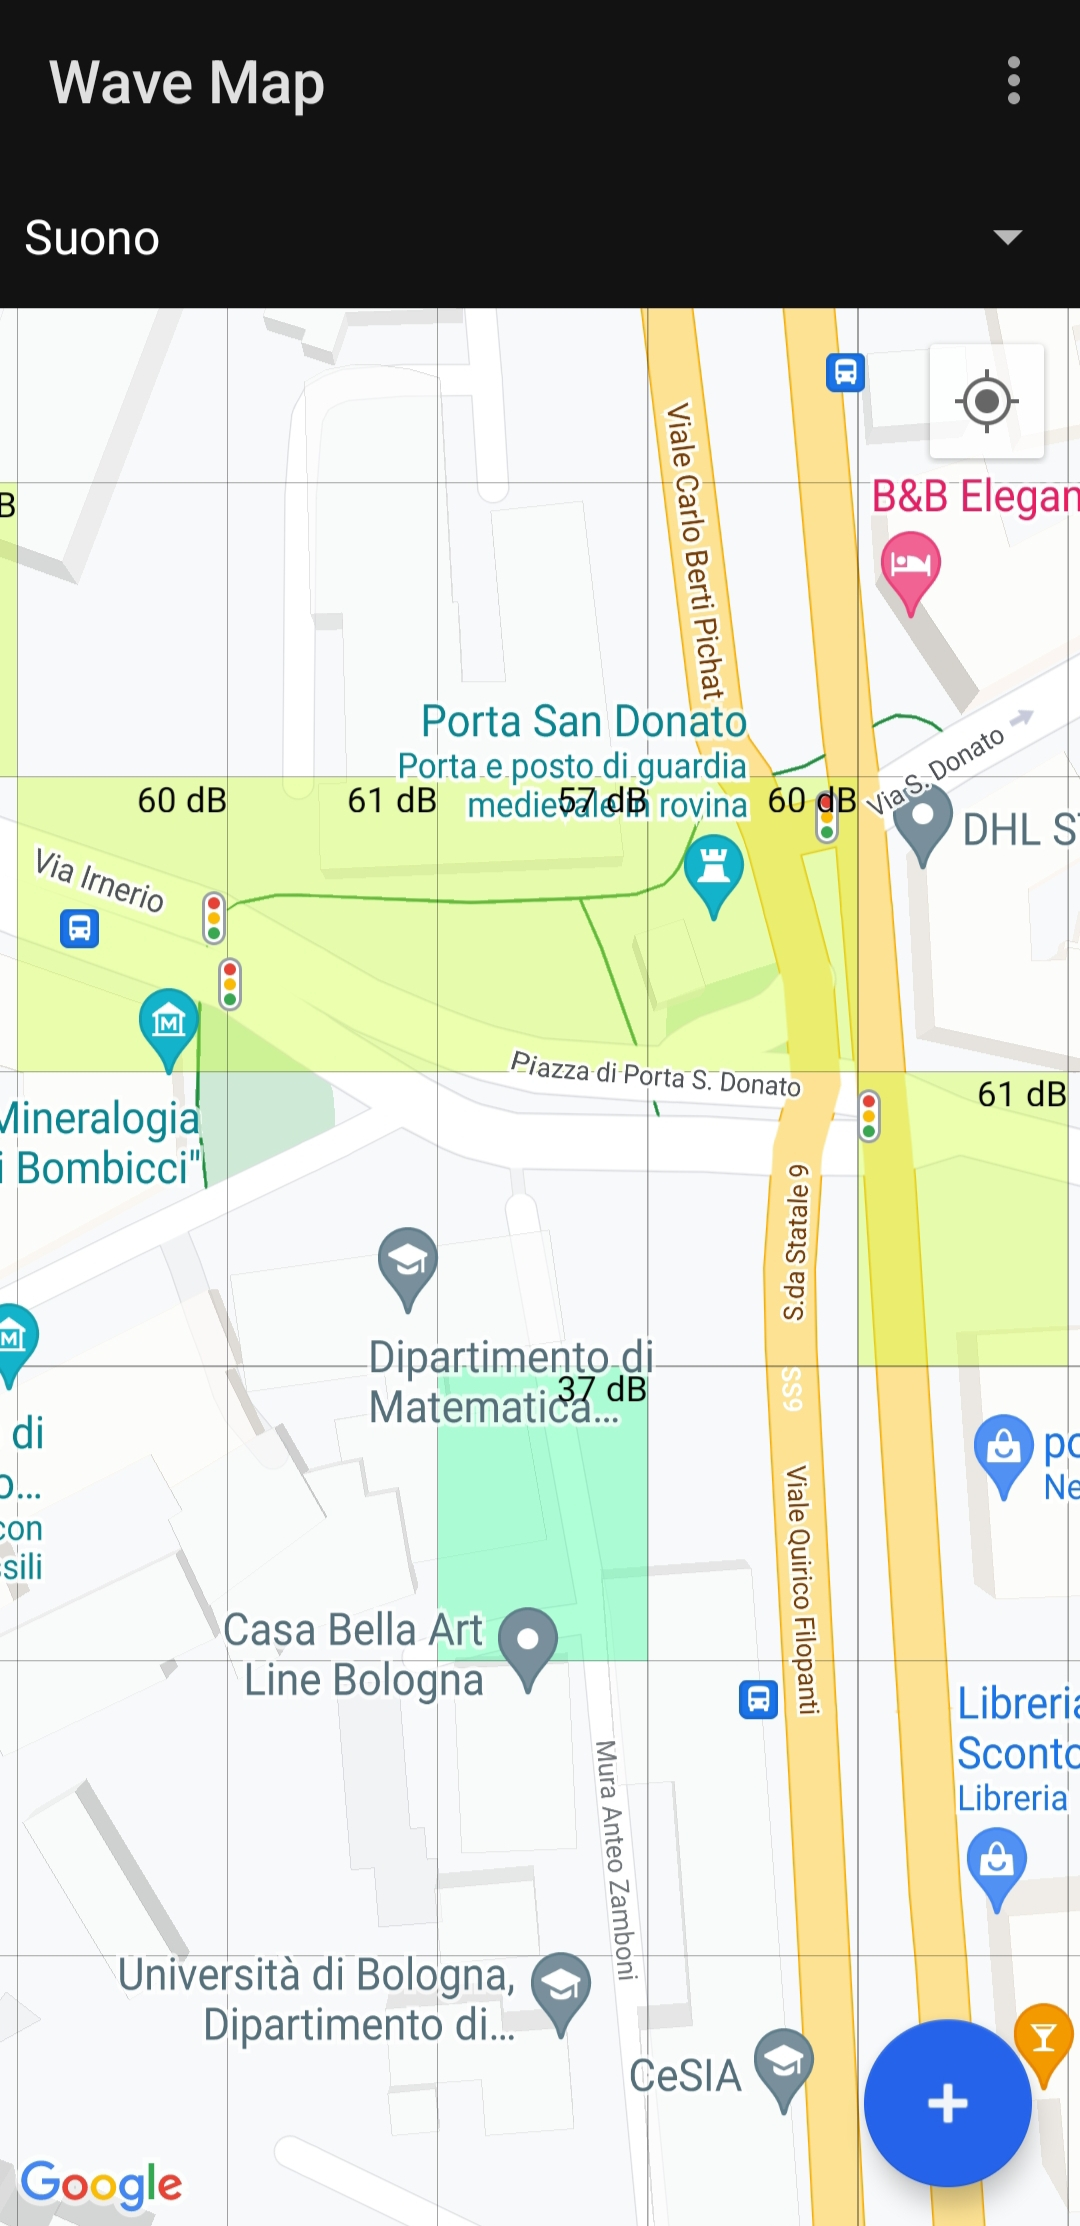
\includegraphics[width=\textwidth]{./img/overview/map_zoom1.jpg}
      \caption*{Suddivisione in 3 range}
    \end{minipage}
    \hspace*{1cm}
    \begin{minipage}[b]{0.25\textwidth}
      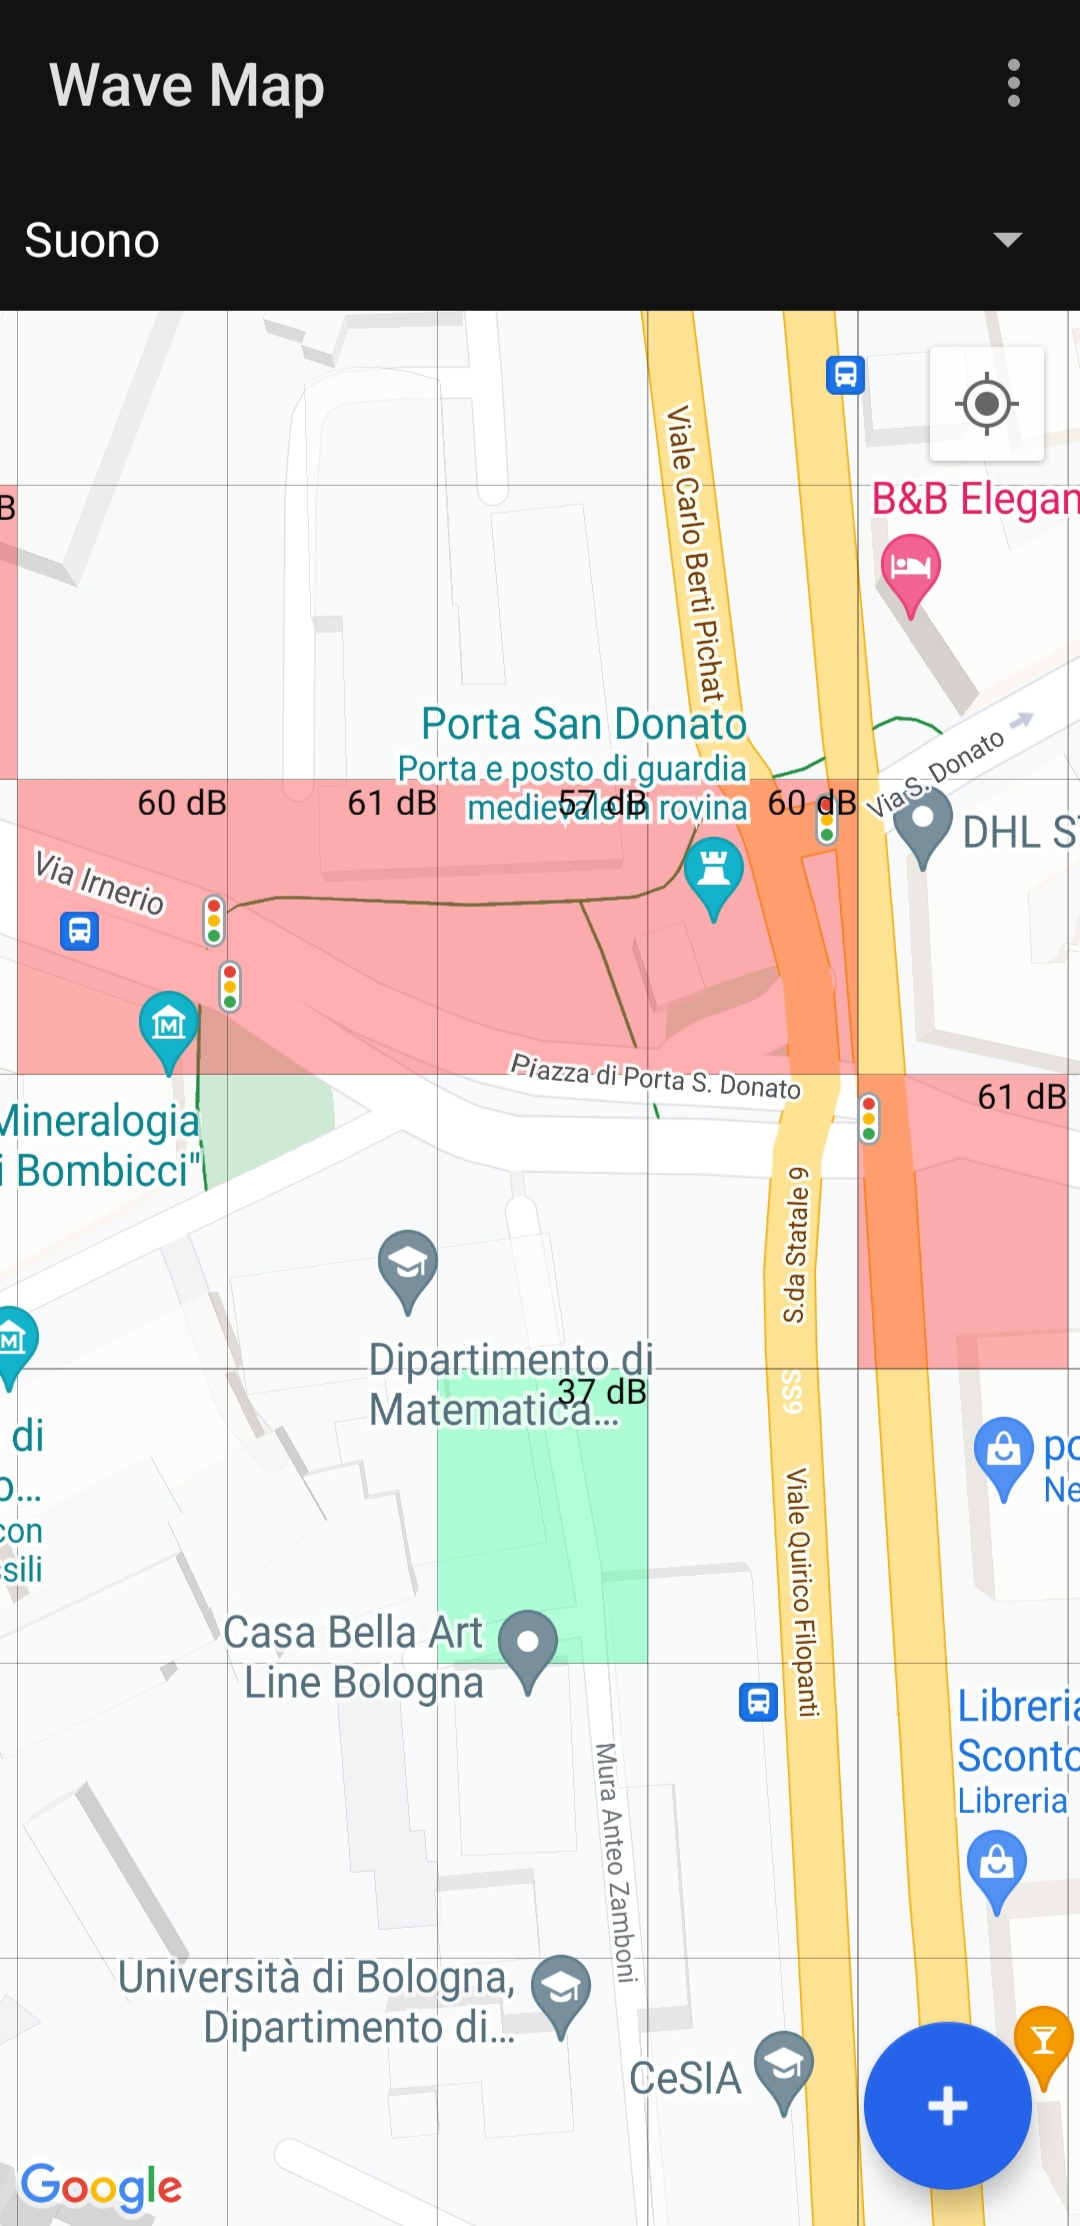
\includegraphics[width=\textwidth]{./img/overview/map_ranges.jpg}
      \caption*{Suddivisione in 2 range}
    \end{minipage}
    \caption{Range misurazioni calcolati algoritmicamente} \label{fig:overview_ranges}
\end{figure}

\begin{figure}[H]
    \centering
    \begin{minipage}[b]{0.25\textwidth}
      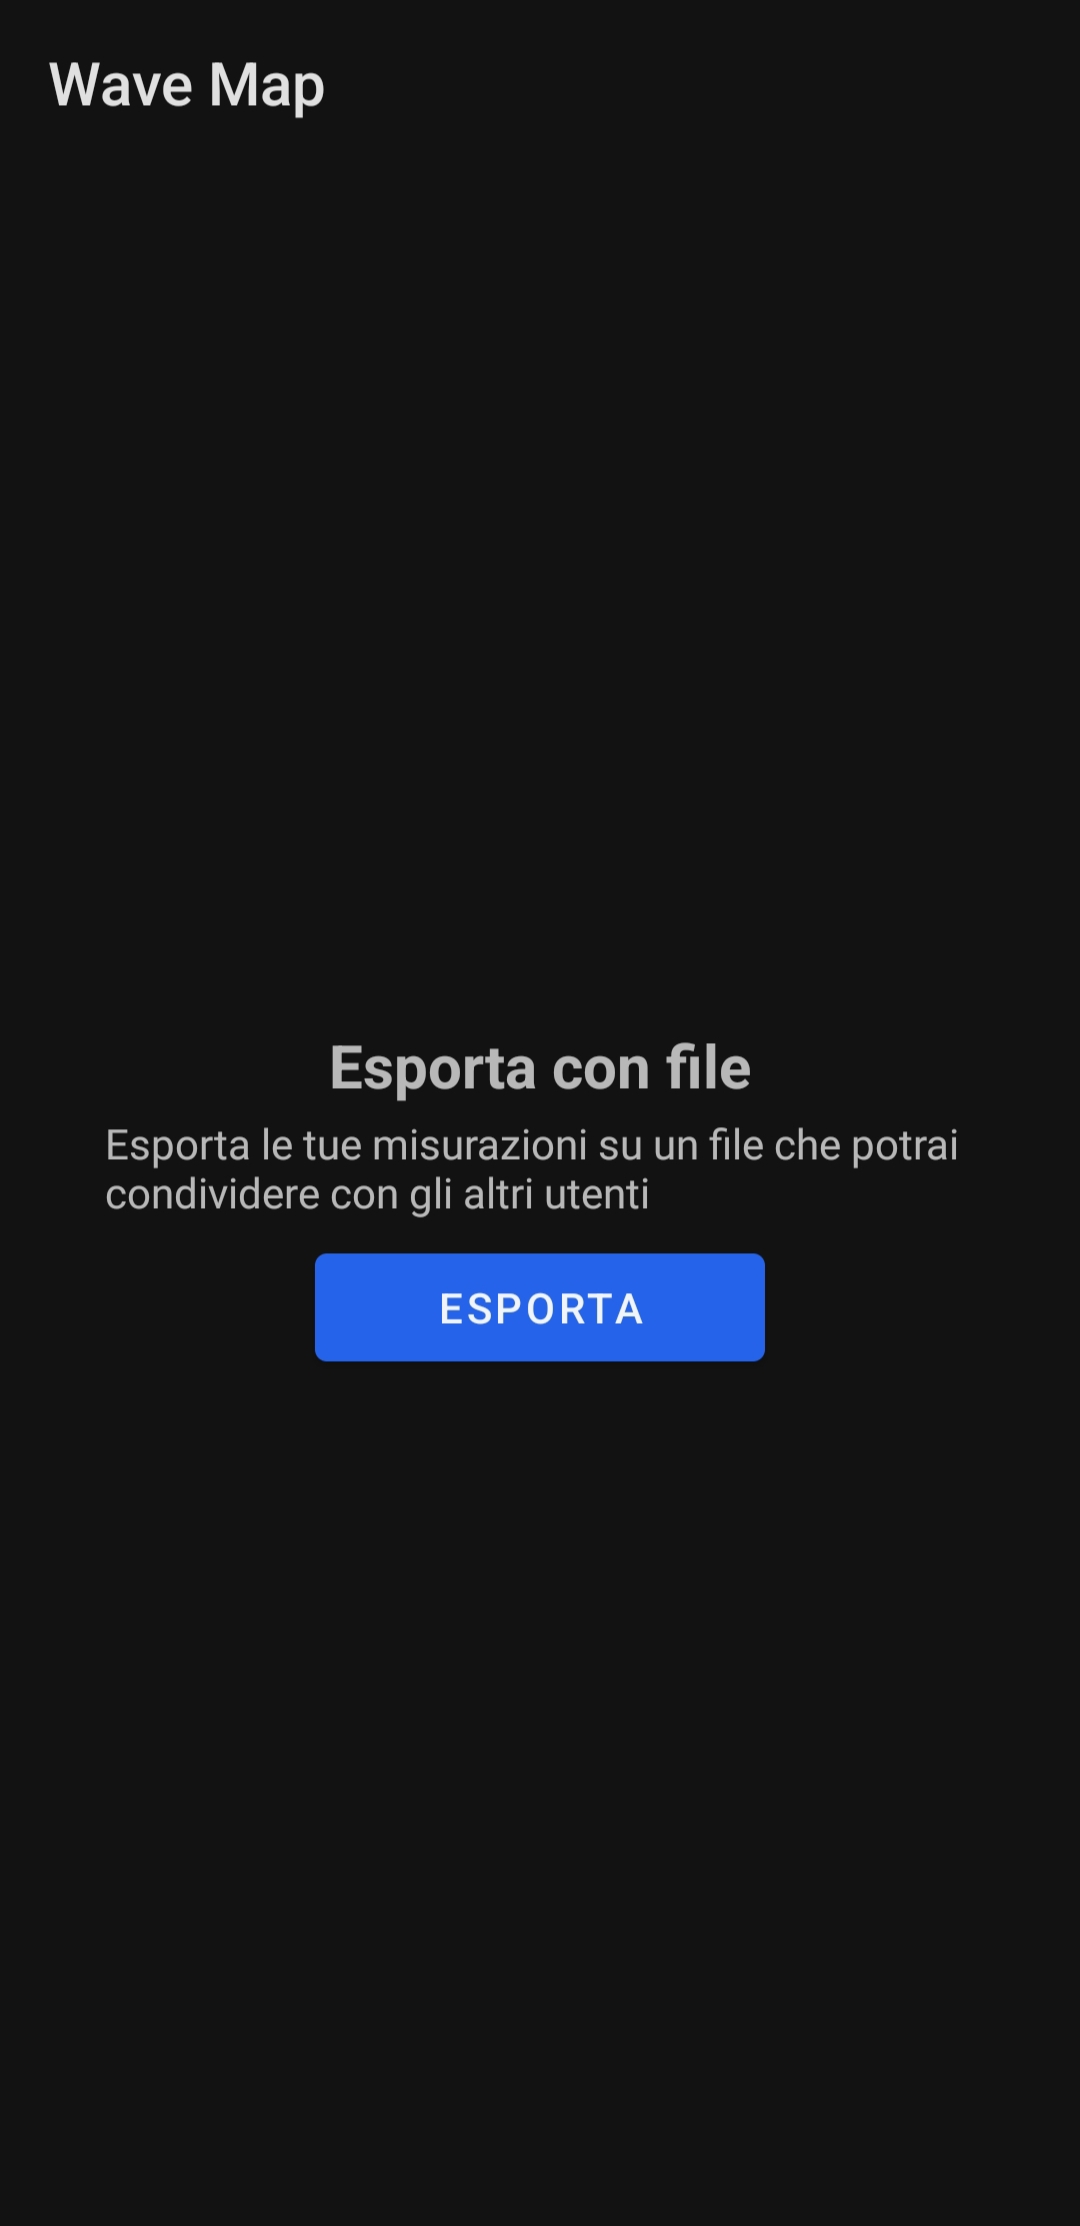
\includegraphics[width=\textwidth]{./img/overview/export1.jpg}
    \end{minipage}
    \begin{minipage}[b]{0.25\textwidth}
      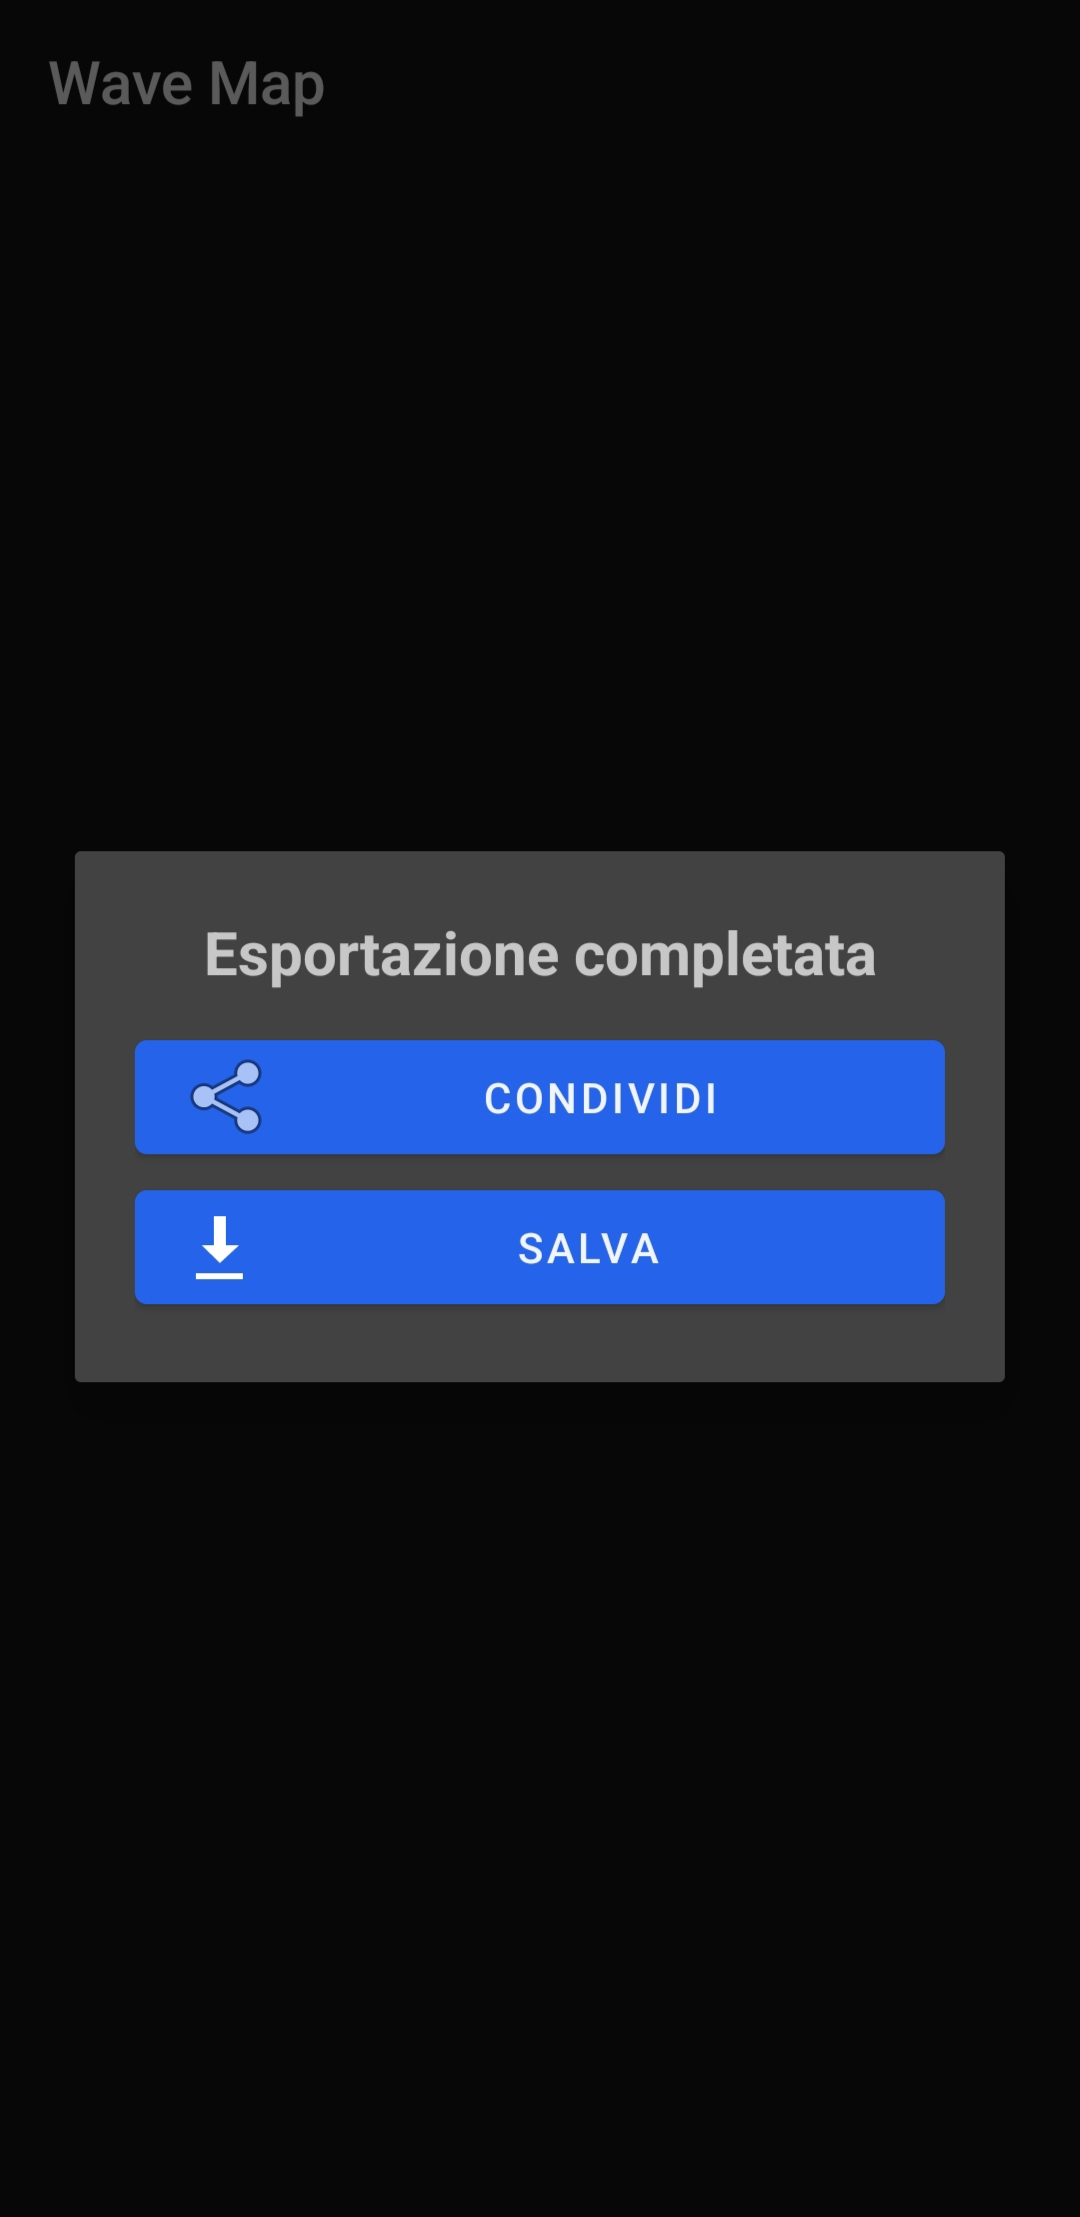
\includegraphics[width=\textwidth]{./img/overview/export2.jpg}
    \end{minipage}
    \hspace*{1cm}
    \begin{minipage}[b]{0.25\textwidth}
      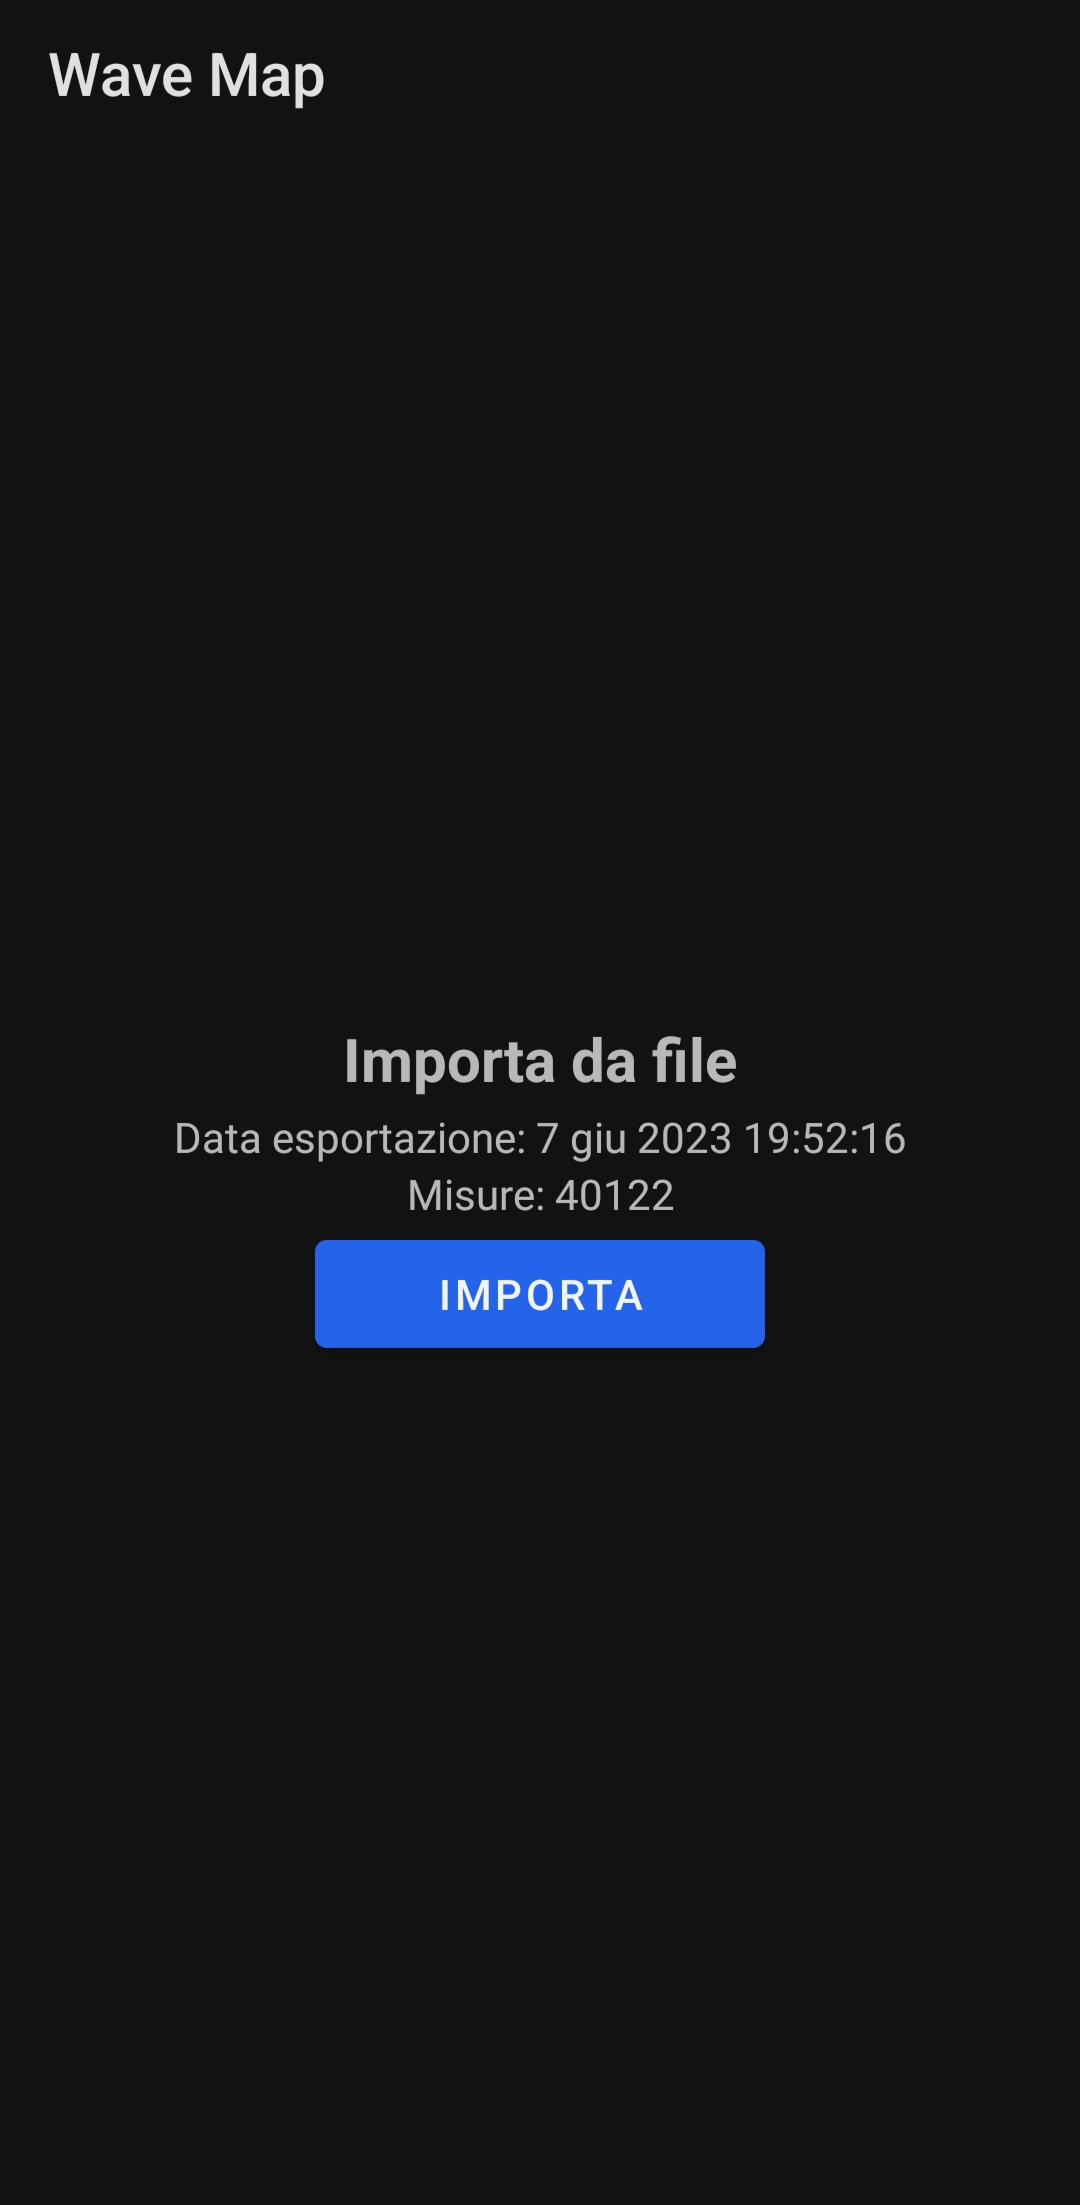
\includegraphics[width=\textwidth]{./img/overview/import.jpg}
    \end{minipage}
    \caption{Esportazione e importazione da file} \label{fig:overview_import_export}
\end{figure}



\section{Scelte progettuali}

\subsection{Informazioni generali}
Il progetto è stato sviluppato come applicazione nativa utilizzando Kotlin. 
Come pattern architetturale è stato scelto l'approccio Model-View-ViewModel, mentre per l'interfacciamento con il database locale è stata utilizzata la libreria \textit{Room}.

Le operazioni asincrone sono state principalmente implementate tramite le \texttt{coroutine}.
Inoltre, per favorire un codice più "lineare", quando possibile, sono state trasformate le funzioni con callback in funzioni \texttt{suspend} utilizzando come wrapper \texttt{suspendCoroutine}.


\subsection{Mappa}
Per la mappa è stato utilizzato \gmaps{} e l'implementazione è contenuta nel fragment \texttt{WaveHeatMapFragment}.

\subsubsection{Generazione cella}
Una cella della mappa rappresenta la misurazione di un'area quadrata\footnote{Esclusa la zona equatoriale, le celle appariranno rettangolari} e la dimensione di quest'ultima scala automaticamente in base al livello dello zoom.

Una cella è descritta dalle coordinate del vertice superiore sinistro (nord-ovest) e a partire da questa vengono calcolate le coordinate degli altri convertendo la dimensione della cella (in metri) in un offset da applicare a latitudine e longitudine.
Per questioni estetiche, gli offset sono approssimati in modo tale che tutte le righe siano allineate verticalmente (\cref{fig:tile_offset}).
\begin{figure}[h]
    \centering
    \begin{minipage}[b]{0.45\textwidth}
      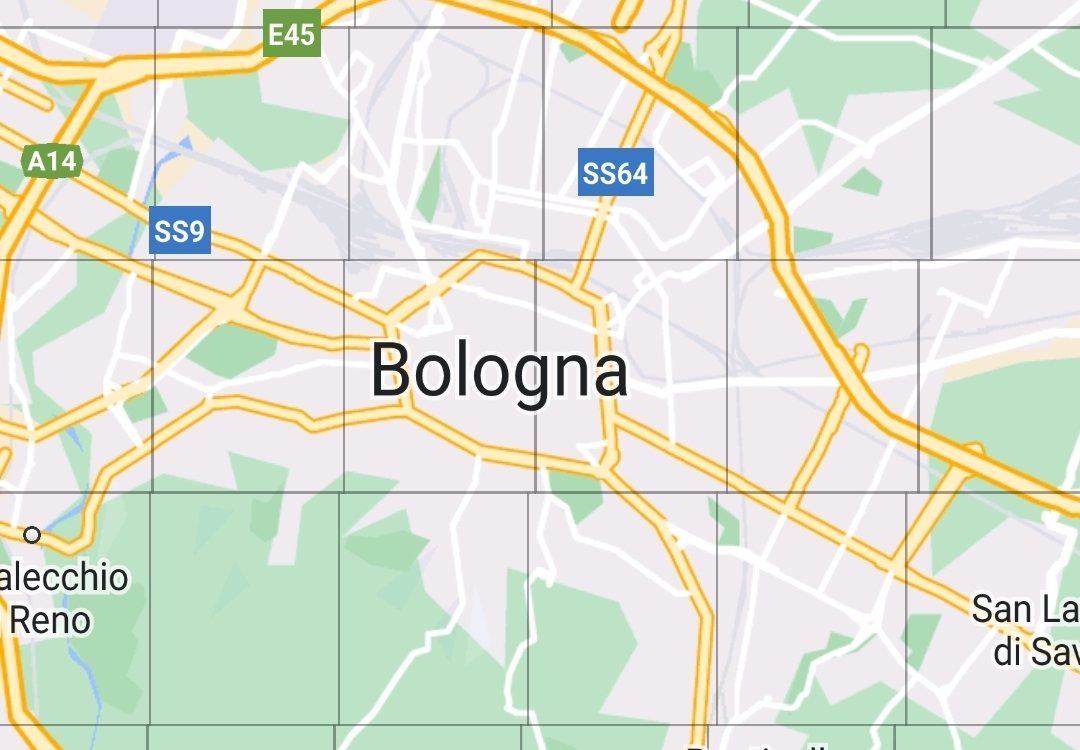
\includegraphics[width=\textwidth]{./img/tile_no_approx.jpg}
    \end{minipage}
    \hfill
    \begin{minipage}[b]{0.45\textwidth}
      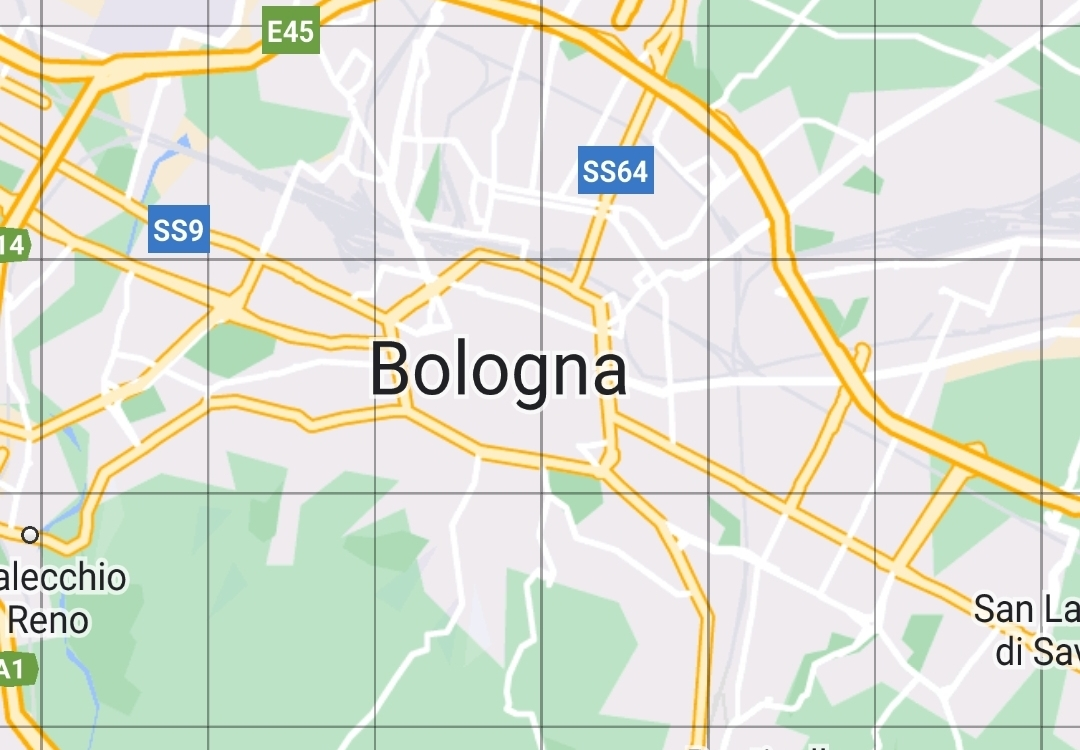
\includegraphics[width=\textwidth]{./img/tile_approx.jpg}
    \end{minipage}
    \caption{Offset calcolati in maniera precisa (sinistra) e approssimata (destra)} \label{fig:tile_offset}
\end{figure}

Il colore di una cella è determinato dal valore e dal tipo di misurazione, e viene impostato in formato HSV modificando il valore della tinta (hue).
Per ciascuna tipologia di misurazione sono specificati gli estremi del range di qualità e il numero di intervalli in cui suddividerlo.
La tinta è quindi determinata collocando il valore della misurazione in uno dei sotto-intervalli del range e selezionando come valore finale l'estremo inferiore (\cref{alg:hue}).

\begin{algorithm}[H]
  \caption{Tinta di una cella}\label{alg:hue}
  \SetAlgoLined
  \SetKwProg{Fn}{fun}{}{end}
  \Fn{\textup{\texttt{{getHue(measure, measure\_range=[$a$, $b$], hue\_range=[$0$, $150$], n\_ranges)}}}}{
    $\texttt{hue} \gets \text{\texttt{measure} scalata da \texttt{measure\_range} a \texttt{hue\_range}}$\\
    $\texttt{hue} \gets \text{\texttt{hue} discretizzata in \texttt{hue\_range} suddiviso in \texttt{n\_ranges} valori}$\\
    return \texttt{hue}
  }
\end{algorithm}

Infine, per ogni cella è presente un'etichetta contenente il valore della misurazione. Poiché \gmaps{} non permette di inserire esplicitamente del testo nella mappa, l'implementazione prevede di generare l'etichetta come un'immagine che viene poi impostata come icona di un marker. Inoltre, la dimensione del testo viene scalata per far in modo che rientri nei limiti della cella.


\subsubsection{Generazione griglia}
La griglia è composta da celle generate relativamente ad una posizione di riferimento. In particolare, in fase di inizializzazione viene designata come cella di riferimento quella che pone la posizione dell'utente al centro e in base a questa è possibile determinare la posizione di tutte le altre celle della mappa. 

Nello specifico, date delle coordinate $(\texttt{pos}_{\texttt{lat}}, \texttt{pos}_{\texttt{lon}})$, per determinare la cella che la contiene si calcola il numero di celle da saltare rispetto a quella di riferimento: 
\begin{equation*}
    \texttt{to\_skip\_tiles}_\texttt{lat} =
        \lceil \frac{\texttt{pos}_{\texttt{lat}} - \texttt{center\_top\_left}_{\texttt{lat}}}{\texttt{latitudeOffset(tile\_length\_meters)}} \rceil
\end{equation*}
\begin{equation*}
    \texttt{to\_skip\_tiles}_\texttt{lon} =
        \lfloor \frac{\texttt{pos}_{\texttt{lon}} - \texttt{center\_top\_left}_{\texttt{lon}}}{\texttt{longitudeOffset(tile\_length\_meters)}} \rfloor
\end{equation*}
Le coordinate del vertice superiore sinistro della cella che contiene $(\texttt{pos}_{\texttt{lat}}, \texttt{pos}_{\texttt{lon}})$ sono quindi:
\begin{equation*}
    \texttt{tile}_\texttt{lat} = \texttt{center\_top\_left}_{\texttt{lat}} + (\texttt{to\_skip\_tiles}_\texttt{lat} \cdot \texttt{latitudeOffset(tile\_length\_meters)})
\end{equation*}
\begin{equation*}
    \texttt{tile}_\texttt{lon} = \texttt{center\_top\_left}_{\texttt{lon}} + (\texttt{to\_skip\_tiles}_\texttt{lon} \cdot \texttt{longitudeOffset(tile\_length\_meters)})
\end{equation*}

Con questo approccio, ogni volta che viene spostata la visuale della mappa, la griglia viene generata iterando a partire dalle coordinate dell'angolo nord-ovest visibile dello schermo, fino a raggiungere l'angolo sud-est. 

In aggiunta, per maggiore efficienza, si tiene traccia delle celle generate in modo da evitare di ridisegnare una cella già presente. Questo meccanismo viene resettato quando viene cambiato il livello di zoom, in quanto tutte le celle già presenti diventano obsolete e vengono cancellate.



\subsection{Raccolta dei dati}

\subsubsection{Struttura e memorizzazione delle misurazioni}
Una misurazione è descritta dall'interfaccia \texttt{WaveMeasure} e contiene il valore della misurazione, un timestamp, la posizione e un flag per indicare se si tratta di una misurazione propria o ottenuta tramite condivisione. 
In aggiunta, è presente un campo per informazioni aggiuntive utile per distinguere alcune tipologie di misurazioni (es. per Wi-Fi e Bluetooth viene salvato il BSSID).

L'interfaccia \texttt{WaveMeasure} viene quindi utilizzata per implementare la classe \texttt{MeasureTable} che descrive la tabella del database dedicata per memorizzare le misurazioni. 
Tutte le misurazioni sono salvate nella stessa tabella e sono differenziate da un campo (\texttt{type}) aggiunto in fase di salvataggio nel database.


\subsubsection{Sampler}
Per la raccolta dei dati è stato introdotto il concetto di \textit{sampler} per gestire in maniera modulare le misurazioni.
Nello specifico, un \textit{sampler} è descritto dalla classe astratta \texttt{WaveSampler} e richiede l'implementazione dei seguenti metodi:
\begin{itemize}
    \item \texttt{sample} per prendere una nuova misurazione.
    \item \texttt{store} per il salvataggio dei dati nel database.
    \item \texttt{retrieve} per la ricerca dei dati note le coordinate dei vertici di una cella della mappa.
\end{itemize}
Inoltre, sono esposte le seguenti funzioni ausiliarie:
\begin{itemize}
    \item \texttt{average} richiama \texttt{retrieve} e restituisce la media dei valori.
    \item \texttt{sampleAndStore} richiama in sequenza \texttt{sample} e \texttt{store}.
\end{itemize}
Per maggiore flessibilità, le misure vengono sempre intese come liste di \texttt{WaveMeasure}. Ciò permette di gestire misurazioni che per loro natura non generano un'unica misurazione (es. Wi-Fi e Bluetooth).

A partire da \texttt{WaveSampler} sono quindi implementati i \textit{sampler} per:
\begin{itemize}
  \item Wi-Fi (\texttt{WiFiSampler}): 
    \begin{itemize}[topsep=0em]
      \item Ottiene la potenza della rete al quale il dispositivo è attualmente connesso tramite il servizio di sistema \texttt{ConnectivityManager}. Per versioni inferiori alla API 29, viene invece utilizzato il \texttt{WifiManager}.
      \item Misura la potenza delle reti circostanti registrando un \texttt{BroadcastReceiver} con filtro \texttt{WifiManager.SCAN\_RESULTS\_AVAILABLE\_ACTION} e richiedendo una scansione completa attraverso il \texttt{WifiManager}.
    \end{itemize}
  \item Bluetooth (\texttt{BluetoothSampler}):
    \begin{itemize}[topsep=0em]
      \item Misura la potenza dei dispositivi accoppiati mediante il \texttt{BluetoothManager}.
      \item Misura la potenza dei dispositivi circostanti registrando un \texttt{BroadcastReceiver} con filtro \texttt{BluetoothDevice.ACTION\_FOUND} e richiedendo al \texttt{BluetoothManager} una scansione completa.
    \end{itemize}
  \item LTE (\texttt{LTESampler}): ottiene la potenza del segnale LTE tramite il \texttt{TelephonyManager}
  \item Suono (\texttt{NoiseSampler}): viene fatta la media di una serie di campionature effettuate utilizzando un \texttt{MediaRecorder}.
\end{itemize}



\subsection{Servizi in background}


\subsection{Condivisione dati}


\subsection{Componenti}
\subsubsection{App principale}
\subsubsection{Impostazioni}
\subsubsection{Condivisione}



\section{Problemi noti}

\subsection{Scansione Wi-Fi}
\subsection{Servizio in background}


\end{document}
